\section{Introduction}

	The aim of this miniproject is to get the experience on implementing two different machine learning methods for solving the same hand-written digits pattern recognition problem. We are supposed to understand and use both error back-propagation gradient descent optimization for a multi-layer perceptron (MLP) and a support vector machine (SVM) method, then apply to the MNIST dataset. So, we can compare the performance for each methods and discuss how and why the results behaved.

\section{Methods}
\begin{enumerate}[(1)]
\item The given .mat files contain training and test sets for the two binary classification. For the multi-layer perceptron (MLP), we are supposed to distinguish between digits 3 and 5 and between digits 4 and 9. Each image of a digit is stored as a vector of length 784. The provided files contain pattern matrices of size n$\times$784, where n is the number of patterns. The training set is used for training the data and updating the parameter, and the test set is used only for evaluation of the final performance.

	The next step for the multi-layer perceptron (MLP) is to split the training part into a training set (2/3) and a validation set (1/3). In the provided training data there are n=6,000 patterns, so after splitting the the size of the training set is 4,000$\times$784 and the test set is 2,000$\times$784.

	The first thing we have to do for machine learning problem is the preprocessing such as loading the datasets in the directory path we created, and then normalizing all of the data to have coefficients between 0 and 1. To do this, we compute the maximum $\alpha_{max}$ and the minimum $\alpha_{min}$ over all coefficients of all training patterns, then substitute each input pattern by the following equation
\begin{align}
x_{normalized}=\frac{1}{\alpha_{max} - \alpha_{min}}(x-\alpha_{min}\mathbf{1})
\end{align}
For the test set, we also normalize all pattern by using the same coefficients $\alpha_{max}$ and $\alpha_{min}$ as stored in the training patterns because we cannot treat and compute the test data even for preprocessing.

\item The final setup of the MLP: the network structure for this project, we use a two-layer MLP, with one hidden and one output layer, use the gating transfer function as the following
\begin{align}
g(a_1,a_2)=a_1 \sigma(a_2),\quad\sigma(x) = \frac{1}{1+e^{-x}}
\end{align}
for the hidden units. The binary classifier and the activation for each layer are given by
\begin{align}
f(x)=\text{sgn}(a^{(2)}(x)),\quad a^{(2)}(x) = \sum_{q=1}^{h_1} w_{q}^{(2)} g(a_{2q-1}^{(1)}, a_{2q}^{(1)})+b^{(2)}\\
a_{k}^{(1)} = \sum_{j=1}^{d} w_{kj}^{(1)}x_{j}+b_{k}^{(1)},\quad k=1,2,\dots,2h_{1}
\end{align}

In the code, we are supposed to minimize the logistic error function, which evaluated the whole training set, is given by
\begin{align}
E_{log}(w)=\frac{1}{n}\sum_{i=1}^n log(1+e^{-t_i a^{(2)}(x_i)})
\end{align}
where the binary training dataset is $D=\{(x_{i},t_{i}),i=1,...,n\}$ and $t_i$ is -1 or 1.
To do this, we have to evaluate by using the error back-propagation gradient descent optimization, which is to take the gradient with respect to the parameters (weight and bias).
For the output layer, the residual is
\begin{align}
\frac{\partial E_{i}}{\partial b^{(2)}}=r^{(2)}=\frac{\partial E_{i}}{\partial a^{(2)}}=-t_{i}\sigma(t_{i}a^{(2)}(x_{i}))\\
\nabla_{w_q^{(2)}} E_{i}=r^{(2)}\cdot\frac{\partial a^{(2)}}{\partial w_{q}^{(2)}} = r^{(2)}\frac{\partial}{\partial w_{q}^{(2)}} (w_{q}^{(2)} g(a_{2q-1}^{(1)},a_{2q}^{(1)})+b^{(2)})=g(a_{2q-1}^{(1)},a_{2q}^{(1)})
\end{align}

For the hidden layer, the residual is given by
\begin{align}
\frac{\partial E_{i}}{\partial a^{(1)}}=\frac{\partial E_{i}}{\partial a^{(2)}}\cdot\frac{\partial a^{(2)}}{\partial g}\cdot\frac{\partial g}{\partial a^{(1)}} =r^{(2)}w^{(2)}g' = r_{k}^{(1)}
\end{align}
The derivative of the transfer function g is $g'(a_1,a_2)=
\begin{cases}
\sigma(a_2)&,  \text{  k is odd}\cr a_1 \sigma(a_2)(1-\sigma(a_2))&,  \text{  k is even}
\end{cases}$

As a result, the residual for the first layer is expressed as $r_{k}^{(1)}=
\begin{cases}
r^{(2)}w^{(2)}\sigma(a_2)&,  \text{  k is odd}\cr r^{(2)}w^{(2)}a_1 \sigma(a_2)(1-\sigma(a_2))&,  \text{  k is even}
\end{cases}$
And the gradient with respect to weight $w_{kj}^{(1)}$ is thus equal to
\begin{align}
\nabla_{w_{kj}^{(1)}} E_{i}=r_k^{(1)}\frac{\partial}{\partial w_{kj}^{(1)}}(w_{kj}^{(1)} x_{j}+b_{k}^{(1)})=r_{k}^{(1)}x_{j}
\end{align}

For updating the new parameter, we ran the gradient descent with momentum which works as follows
\begin{align}
\Delta w_i=-\eta(1-\mu)\nabla_{w_i}E+\mu\Delta w_{i-1}
\end{align}
denoted by $\Delta w_i=w_{i+1}-w_i$ the update done in iteration i.

We can test if the backpropagation code for the gradient computation is bug-free or not. For the logistic error function E(w) of a single weight w, the gradient of error is
$g(w)=E'(w)=dE/dw$
Gradient testing will be done by comparing the result of gradient g(w) with symmetric finite-difference approximation that is the evaluation of the error function at two other points that are very close to w, given by
\begin{align}
g(w)\simeq\frac{E(w+\epsilon)-E(w-\epsilon)}{2\epsilon}
\end{align}
for a very small $\epsilon > 0$ (we used $\epsilon = 0.001$)

We have tested that the above equation satisfied. It means that our backpropagation code works.
 
To select the best parameters, we ran the MLP algorithm with the various parameters of the number of hidden units $h_{1}=10,20,...,100$, the learning rate $\eta=0.01,0.03,0.1,0.3,1,3,9$ and the momentum term $\mu={0.1,0.2,...,1.0}$ and stored the logistic error in the form of matrices with 4-dimension depending on each parameters h1,$\eta$, $\mu$ and iterations (N=50). Next, we see the effects of each parameters by fixing the remaining parameters for every iterations.
	\begin{figure}[htbp]
		\centering
		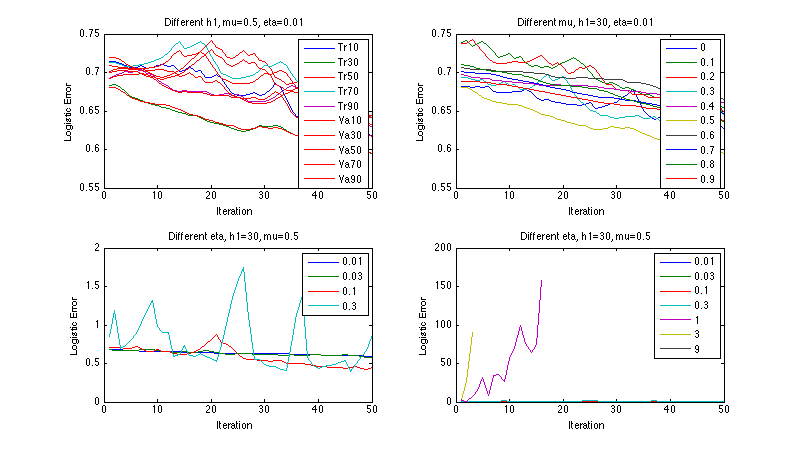
\includegraphics[width=0.99\textwidth]{plots/h1,mu,eta.png}
		\caption{Model Selection (1)different $h_1$ (2)different $\mu$ (3)different $\eta=0.01-0.3$ (3)different $\eta=0.01-9$ for digits 3and5}
		\label{fig:h1,mu,eta}
	\end{figure}
The experiment tells us that if we do not select the parameter appropriately, we will face some problems. According to the figure \ref{fig:h1,mu,eta}, we can see the error with different number of hidden units $h_1$. It showed about the overfitting problem obviously that the higher $h_1$ is, the larger the error is and the training and validation error are oscillated and its difference is pretty larger. Compared to $h_{1}=30$, there is almost no difference between two errors. Both are almost fit exactly and converge to 0.

In the same figure, a small learning rate $\eta$ like 0.01, the error decreases slowly, which means slow convergence during gradient descent. Also, while  $\eta=0.3$, it has a faster convergence. After a certain point, increasing $\eta$=3 or 9 will no longer increase the convergence speed. Similarly, if the momentum term $\mu$ is too small, the convergence speed is too fast and eventually does not converge due to oscillation (zig-zagging). The results follow from the theory we have learnt.

For each selection, we selected the best parameter that gives the minimum logistic error has no over fitting and not too fast convergence speed. As a result, for example we choose the number of hidden units $h_1=30$, the learning rate $\eta=0.01$ and the momentum term $\mu=0.5$ for digits 3 and 5 binary classification.

\item For each binary subtasks, we used the different parameters. The method for model selection, and the chosen parameters and its plots for digits 3 and 5 has been shown in the previous part. We conclude the chosen parameters as the following.\\
The 3 and 5 binary subtask, $h_1=30$, $\eta=0.01$, $\mu=0.5$ . \\
The 4 and 9 binary subtask, $h_1=70$, $\eta=0.01$, $\mu=0.3$ . \\ 
The plots for choosing the parameter for 4 and 9 binary subtask has been depicted in figure \ref{fig:}

\item To see one example of overfitting, let us use a large number of hidden units $h_1$ (says, 100) and do not use the early stopping. Then plot the graph to show the comparison between training and validation error as in figure \ref{fig:overfitting}
	\begin{figure}[htbp]
		\centering
		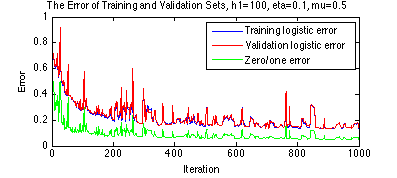
\includegraphics[width=0.99\textwidth]{plots/overfitting.png}
		\caption{The example of overfitting}
		\label{fig:overfitting}
	\end{figure}
\end{enumerate}

\section{Result and Discussion}
\begin{enumerate}
\item By learning the multi-layer perceptron (MLP), we got the training set logistic error, the validation set logistic error, and the validation set (zero/one) error as a function of the epoch number
\begin{align}
\frac{1}{m}\sum_{j=1}^{m} \I{t_{j} a^{(2)}(x_j)\le{0}}. 
\end{align}
The error curves for digits 3 and 5, and 4 and 9 binary classification have been shown in figure \ref{fig:3error}(1) and \ref{fig:3error}(2) respectively.

	\begin{figure}[htbp]
		\centering
		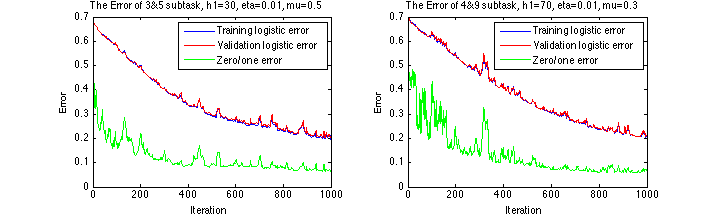
\includegraphics[width=0.99\textwidth]{plots/3error.png}
		\caption{The training set logistic error, the validation set logistic error, and the zero/one error for each iterations for digits 3and5 (1) and 4and9 (2)}
		\label{fig:3error}
	\end{figure}
	
\item After learning MLP, for 3and5 subtask the training error is 0.2005, so the accuracy is 99.7995\%. for 4and9 subtask, the training error and the accuracy are 0.2095 and 99.7905\%, we got the latest updated parameters (weight and bias). We used it to compute the error and the activation over the whole test dataset. Then, we evaluate the misclassified data by computing $t_i a^{(2)} (x_i)$ for each pattern. For digits 3 and 5 binary classification, the result is illustrated in figure \ref{fig:testerror}(1), the standard deviation is $\sigma=1.7550$ and the error of test set is 0.1855 (accuracy=99.8145\%). For digits 4 and 9 binary classification, the result is illustrated in figure \ref{fig:testerror}(2),the standard deviation is $\sigma=2.4752$ and the error of test set is 1.1046 (accuracy=98.8954\%). 
The figures showed that the more we trained the data, the more $t_i a^{(2)} (x_i)$ converges to zero. It means that the classification problem works more accurately.
	\begin{figure}[htbp]
		\centering
		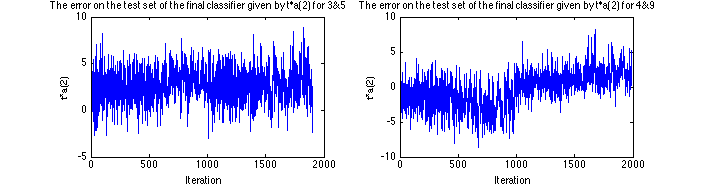
\includegraphics[width=0.99\textwidth]{plots/testerror.png}
		\caption{The computation of the average of $t_i a^{(2)} (x_i)$ for each iterations for digits 3and5 (1) and 4and9 subtask (2)}
		\label{fig:testerror}
	\end{figure}
	
\item Let us give the example of digits 3 and 5 binary subtask. For each run, in the patterns which are misclassified, we stored the values $t_i a^{(2)} (x_i)$ which has largest negative and close to zero. Then, we separately plot the graph in figure \ref{fig:largest_closetozero}.

	\begin{figure}[htbp]
		\centering
		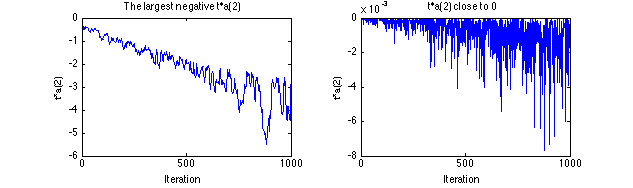
\includegraphics[width=0.99\textwidth]{plots/largest_closetozero.png}
		\caption{$t_i a^{(2)} (x_i)$ which has (1) largest negative and (2) close to zero}
		\label{fig:largest_closetozero}
	\end{figure}

\end{enumerate}